\section{Infrastruktur}
\begin{figure}
    \centering
    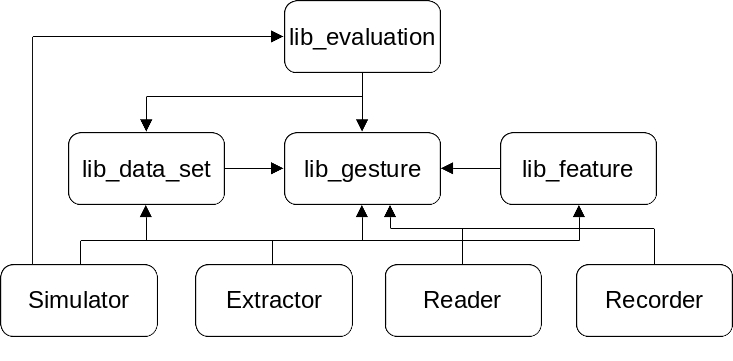
\includegraphics[width=0.75\linewidth]{images/architecture_overview.jpg}
    \caption{Abhängigkeitein der einzelnen Module.}
    \label{fig:architecture_overview}
\end{figure}
Der Kern der Arbeit war es viele Verschiedene Feature und Konfigurationen der Entscheidungsbäume zu untersuchen und zu testen. Aus diesem Grund habe ich es als nötig erachtet eine umfangreiche und dokumentierte Infrastruktur
zu schaffen, die die Auswertung meiner Arbeit und folgenden Arbeiten vereinfacht. Die Infrastruktur umfasst die Erstellung eines Datenmodels und das Auswerten von Datenmengen unter verschiedenen Parsingmethoden.
Außerdem wird die Generierung von synthetischen Daten vereinfacht und eine leicht zu erweiternde Architektur bereitgestellt um Feature zu definieren. All diese Funktionalitäten sind in Bibliotheken verpackt,
die leicht in eigene Projekte zu integrieren sind (siehe Abbildung \ref{fig:architecture_overview}). Darauf aufbauend wurden außerdem einige Programme erstellt, um den Arbeitsablauf zu vereinfachen.
\subsection{lib\_gesture}

\subsection{lib\_feature}
\begin{lstlisting}[label=lst:FeatureInterface,caption={Interface, um ein Feature zu implementieren.}]
pub trait Feature {
    fn calculate(gesture: &Gesture) -> Self where Self: Sized;
    fn marshal(&self) -> String;
}
\end{lstlisting}
\texttt{lib\_feature} bietet ein einfaches Interface an um Feature mit einer Geste (siehe Listing \ref{lst:FeatureInterface}) zu implementieren. Zurzeit sind 28 verschiedene Feature implementiert.
\subsection{lib\_data\_set}

\subsection{lib\_evaluation}

\subsection{Simulator}

\subsection{Extractor}
Der \texttt{Extractor} extrahiert aus spezifizierten Datenmengen die definierten Features und exportiert diese in Dateien, sodass sie von dem Model zum trainieren genutzt werden können. Optional kann die Datenmenge durch
sythetische Daten erweitert werden.
\subsection{Reader}
Der \texttt{Reader} gibt den seriellen Datenstrom des Arduino aus.
\subsubsection{Gesture Recorder}